\documentclass[nooutcomes]{ximera}
%\documentclass[space,handout,nooutcomes]{ximera}

% For preamble materials

\usepackage{pgf,tikz}
\usepackage{mathrsfs}
\usetikzlibrary{arrows}
\usepackage{framed}
\usepackage{amsmath}
\pgfplotsset{compat=1.17}

\def\fixnote#1{\begin{framed}{\textcolor{red}{Fix note: #1}}\end{framed}}  % Allows insertion of red notes about needed edits
%\def\fixnote#1{}

\def\detail#1{{\textcolor{blue}{Detail: #1}}}   

\pdfOnly{\renewenvironment{image}[1][]{\begin{center}}{\end{center}}}

\graphicspath{
  {./}
  {chapter1/}
  {chapter2/}
  {chapter4/}
  {proofs/}
  {graphics/}
  {../graphics/}
}

\newenvironment{sectionOutcomes}{}{}


%%% This set of code is all of our user defined commands
\newcommand{\bysame}{\mbox{\rule{3em}{.4pt}}\,}
\newcommand{\N}{\mathbb N}
\newcommand{\C}{\mathbb C}
\newcommand{\W}{\mathbb W}
\newcommand{\Z}{\mathbb Z}
\newcommand{\Q}{\mathbb Q}
\newcommand{\R}{\mathbb R}
\newcommand{\A}{\mathbb A}
\newcommand{\D}{\mathcal D}
\newcommand{\F}{\mathcal F}
\newcommand{\ph}{\varphi}
\newcommand{\ep}{\varepsilon}
\newcommand{\aph}{\alpha}
\newcommand{\QM}{\begin{center}{\huge\textbf{?}}\end{center}}

\renewcommand{\le}{\leqslant}
\renewcommand{\ge}{\geqslant}
\renewcommand{\a}{\wedge}
\renewcommand{\v}{\vee}
\renewcommand{\l}{\ell}
\newcommand{\mat}{\mathsf}
\renewcommand{\vec}{\mathbf}
\renewcommand{\subset}{\subseteq}
\renewcommand{\supset}{\supseteq}
%\renewcommand{\emptyset}{\varnothing}
%\newcommand{\xto}{\xrightarrow}
%\renewcommand{\qedsymbol}{$\blacksquare$}
%\newcommand{\bibname}{References and Further Reading}
%\renewcommand{\bar}{\protect\overline}
%\renewcommand{\hat}{\protect\widehat}
%\renewcommand{\tilde}{\widetilde}
%\newcommand{\tri}{\triangle}
%\newcommand{\minipad}{\vspace{1ex}}
%\newcommand{\leftexp}[2]{{\vphantom{#2}}^{#1}{#2}}

%% More user defined commands
\renewcommand{\epsilon}{\varepsilon}
\renewcommand{\theta}{\vartheta} %% only for kmath
\renewcommand{\l}{\ell}
\renewcommand{\d}{\, d}
\newcommand{\ddx}{\frac{d}{dx}}
\newcommand{\dydx}{\frac{dy}{dx}}


\usepackage{bigstrut}


%\usepackage{tikz}


\title{Similarity}
\author{Bart Snapp and Brad Findell}
\begin{document}
\begin{abstract}
Short-answer problems about similarity. 
\end{abstract}
\maketitle




%To define a translation, rotation, or reflection, we indicate the image of a generic point $P$ under the transformation as specified.  
%
%Under a rotation about center $O$ counterclockwise by an angle $\theta$, the image of $P$ is 
%a point $Q$ so that $OQ = OP$ and $m\angle POQ = \theta$, measured counterclockwise 
%from $\overrightarrow{OP}$ to $\overrightarrow{OQ}$.  If $P = O$ then $Q=O=P$.  % if $\theta<0$ 
%
%Under a translation by the distance and direction from $A$ to $B$, the image of $P$ is a point $Q$ so 
%that $\overline{PQ} \parallel \overline{AB}$, $PQ=AB$, and $\overrightarrow{PQ}$ is in the same direction as $\overrightarrow{AB}$.  
%
%Under a reflection about a line $\ell$, if $P$ is on $\ell$, then $P$ is mapped to itself.  If $P$ is not on $\ell$, then the image of $P$ is a point $Q$ so that $\ell$ is the perpendicular bisector of $\overline{PQ}$.  
%

\begin{question}
\textbf{Definition.} Under a \textbf{dilation} about center $O$ and scale factor $r>0$, the image of $P$ is 
a point $Q$ so that $Q$ lies on \wordChoice{\choice{segment}\choice[correct]{ray}\choice{line}} 
$\answer[format=string]{OP}$ % $\overrightarrow{OP}$ 
and $OQ=\answer[format=string]{rOP}$.  The image of $O$ is $\answer[format=string]{O}$. 
\end{question}


\begin{question}
Describe, both informally and formally, what it means to say two figures are congruent.
\begin{freeResponse}
\end{freeResponse}
\begin{hint}
\textbf{Informally:}  Two figures are congruent if one can be ``placed upon'' the other so that the figures match exactly.  This is called the ``principle of superposition.''  

\textbf{Formally:}  Two figures are congruent if there is a sequence of basic rigid motions that maps one onto the other.  
\end{hint}
\end{question}

\begin{question}
Describe, both informally and formally, what it means to say two figures are similar.
\begin{freeResponse}
\end{freeResponse}
\begin{hint}
\textbf{Informally:}  Two figures are similar if they have the same shape.  With moving and scaling (zooming in or out), one can be placed on another so that the figures match exactly.    

\textbf{Formally:}  Two figures are similar if there is a sequence of basic rigid motions and dilations that maps one onto the other.  
\end{hint}
\end{question}


\begin{question}
Compare and contrast the ideas of \textit{equal triangles},
  \textit{congruent triangles}, and \textit{similar triangles}.
\begin{freeResponse}
\end{freeResponse}
\begin{hint}
Two triangles are equal if they are the same sets of points.  For example, you could write $\triangle ABC = \triangle BCA$ because they are the same triangle, but this notation is misleading and rarely used.  

Congruence and similarity are defined above.  Two triangles that are congruent have the same angles measures and side lengths.  Two triangles that are similar, it turns out, have the same angle measures.  
\end{hint}
\end{question}

\begin{question}
A student says that any two rectangles are similar because all the angles are the same.  Is the student correct?  
\wordChoice{\choice{Yes.}\choice[correct]{No.}\choice{Not enough information.}} Explain. 
\begin{freeResponse}
\end{freeResponse}
\begin{feedback}
Two rectangles are similar only if there is a single $\answer[format=string]{scale factor}$ (two words) that works for both the length and width.  Angles alone are not enough for quadrilaterals.  
\end{feedback}
\end{question}


\begin{question}
Suppose $\triangle ABC \sim \triangle XYZ$.  Complete the following equation relating ratios \textbf{within} the figures: 
\[
\frac{AB}{\answer{BC}} = \frac{\answer{XY}}{YZ}.  
\]
Complete the following equation relating ratios \textbf{between} (or across) the figures: 
\[
\frac{AB}{\answer{XY}} = \frac{\answer{BC}}{YZ}.  
\]
A ratio between (or across) corresponding lengths from two similar figures is called a $\answer[format=string]{scale}$ factor.  
\end{question}


\begin{question}
Are all equilateral triangles are similar to each other?  
\wordChoice{\choice[correct]{Yes.}\choice{No.}\choice{It depends.}} Explain.  
\begin{freeResponse}
\end{freeResponse}
\begin{feedback}[correct]
Equilateral triangles have interior angles that all measure $\answer{60}$ degrees.  So all equilateral triangles are similar to one another by AAA similarity.  
\end{feedback}
\end{question}

\begin{question}Are all isosceles right triangles similar to each other? 
\wordChoice{\choice[correct]{Yes.}\choice{No.}\choice{It depends.}} Explain.  
\begin{freeResponse}
\end{freeResponse}
\begin{feedback}[correct]
Isosceles right triangles have interior angles that measure $\answer{45}$, $\answer{45}$, and $90$ degrees.  So all equilateral triangles are similar to one another by AAA similarity.  
\end{feedback}
\end{question}

\begin{question}
Explain why when given a right triangle, the altitude of the
  right angle divides the triangle into two smaller triangles each
  similar to the original right triangle.
\begin{freeResponse}
\end{freeResponse}
\begin{hint}
Each of the two smaller triangles has a has a right angle and shares an acute angle with the original triangle.  By AA similarity, each of the smaller triangles is similar to the large triangle, and thus the three triangles must be similar to one another.  
\end{hint}
\end{question}

\begin{question}
The following sets contain lengths of sides of similar
  triangles. Solve for all unknowns---give all solutions. In each case
  explain your reasoning.
\begin{enumerate}
%\item $\{3,4,5\}$, $\{6,8,x\}$
%\item $\{3,3,5\}$, $\{9,9,\x\}$
\item $\{3,4,5\}$, $\{6,8,\answer{10}\}$
\item $\{3,3,5\}$, $\{9,9,\answer{15}\}$
%\item $\{5,5,x\}$, $\{10,4,y\}$
%\item $\{5,5,x\}$, $\{10,8,y\}$
%\item $\{3,4,x\}$, $\{4,5,y\}$ 
\end{enumerate}
\end{question}

\begin{question}
A \textit{Pythagorean Triple}\index{Pythagorean Triple} is a set
  of three positive integers $\{a,b,c\}$ such that $a^2 + b^2 =
  c^2$. Write down an infinite list of Pythagorean Triples. Explain
  your reasoning and justify all claims.
\begin{freeResponse}
\end{freeResponse}
\begin{hint}
Scale any Pythagorean triple by an integer scale factor greater than 1, and you have another Pythagorean triple.  For example, \{3, 4, 5\} is a Pythagorean triple, and so is \{$3n$, $4n$, $5n$\} if $n \ge 1$ is an integer.  
\end{hint}
\end{question}

\begin{question}
Here is a right triangle, \textbf{not} drawn to scale:
\begin{image}
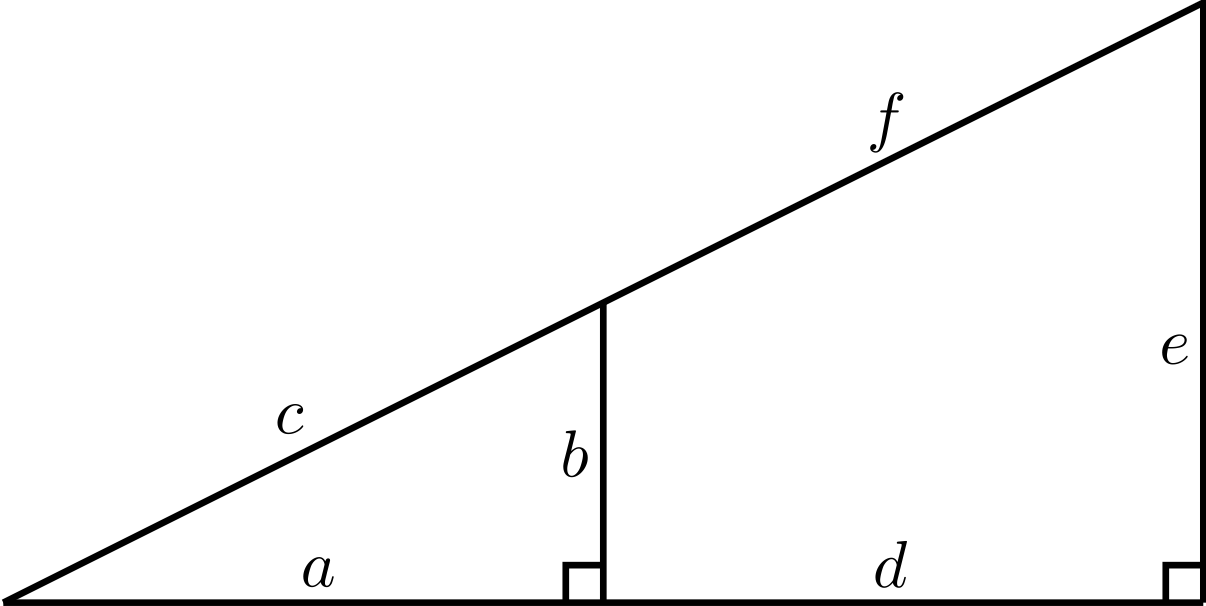
\includegraphics{origamiSimQ.png}
\end{image}
Solve for all unknowns in the following cases.  Note:  To enter, say, $\sqrt{3}$, type \texttt{sqrt(3)} or use the Math Editor. 
\begin{enumerate}
\item $a = 3$, $b = \answer{1}$, $c = \answer{\sqrt{10}}$, $d = 12$, $e = 5$, $f = \answer{4 \sqrt{10}}$
\item $a = \answer{12/5}$, $b = 3$, $c = \answer{3\sqrt{41}/5}$, $d =8$, $e = 13$, $f = \answer{2\sqrt{41}}$
\item $a = 7$, $b = 4$, $c = \answer{\sqrt{65}}$, $d =\answer{49/4}$, $e = 11$, $f = \answer{7\sqrt{65}/4}$
\item $a = 5$, $b = 2$, $c = \answer{\sqrt{29}}$, $d =6$, $e = \answer{22/5}$, $f = \answer{6\sqrt{29}/5}$
\end{enumerate}
% In each case explain your reasoning.
\end{question}

\begin{question}
Suppose you have two similar triangles. What can you say about
  the area of one in terms of the area of the other? Be specific and
  explain your reasoning.
\begin{freeResponse}
\end{freeResponse}
\begin{hint}
If the triangles are similar with a scale factor of $r$, then the ratio of their areas is $\answer{r^2}$. 
\end{hint}
\end{question}

\begin{question}
During a solar eclipse we see that the apparent diameter of the
  Sun and Moon are nearly equal. If the Moon is around $240,000$ miles
  from Earth, the Moon's diameter is about $2000$ miles, and the Sun's
  diameter is about $865,000$ miles how far is the Sun from the Earth?
%\begin{enumerate}
%\item Draw a relevant (and helpful) picture showing the important
%  points of this problem.
%\item Solve this problem, be sure to explain your reasoning.
%\end{enumerate}

Distance to sun $\approx \answer{(865000/2000)240000}$ miles. 
\end{question}

\begin{question}
When jets fly above $8,000$ meters in the air they form a vapor
  trail. Cruising altitude for a commercial airliner is around $10,000$
  meters. One day I reached my arm into the sky and measured the
  length of the vapor trail with my hand---my hand could just span the
  entire trail. If my hand spans $9$ inches and my arm extends $25$
  inches from my eye, how long is the vapor trail in \textbf{kilometers}? 
  %Explain your reasoning.
%\begin{enumerate}
%\item Draw a relevant (and helpful) picture showing the important
%  points of this problem.
%\item Solve this problem, be sure to explain your reasoning.
%\end{enumerate}

Length of vapor trail $\approx \answer{(10/25)9}$ km. 
\end{question}

%\begin{question}
%David proudly owns a 42 inch (measured diagonally) flat screen
%  TV. Michael proudly owns a 13 inch (measured diagonally) flat screen
%  TV. Dave sits comfortably with his dog Fritz at a distance of 10
%  feet. How far must Michael stand from his TV to have the ``same''
%  viewing experience?  Explain your reasoning.
%%\begin{enumerate}
%%\item Draw a relevant (and helpful) picture showing the important
%%  points of this problem.
%%\item Solve this problem, be sure to explain your reasoning.
%%\end{enumerate}
%
%Standing distance $\approx \answer{(13/42)10}$ feet.  
%\end{question}

%\begin{question}
%You love IMAX movies. While the typical IMAX screen is 72 feet
%  by 53 feet, your TV is only a 32 inch screen---it has a 32 inch
%  diagonal. How close do you have to sit to your screen to simulate
%  the IMAX format? Explain your reasoning.
%\begin{enumerate}
%\item Draw a relevant (and helpful) picture showing the important
%  points of this problem.
%\item Solve this problem, be sure to explain your reasoning.
%\end{enumerate}
%\end{question}

%\begin{question}
%Here is a personal problem: Suppose you are out somewhere and
%  you see that when you stretch out your arm, the width of your thumb
%  is the same apparent size as a distant object. How far away is the
%  object if you know the object is:
%\begin{enumerate}
%\item 6' long (as tall as a person).
%\item 16' long (as long as a car).
%\item 40' long (as long as a school bus).
%\item 220' long (as long as a large passenger airplane).
%\item 340' long (as long as an aircraft carrier).
%\end{enumerate}
%Explain your reasoning.
%\begin{freeResponse}
%\begin{hint}
%\end{hint}
%\end{freeResponse}
%\end{question}
%
%\begin{question}
%I was walking down Woody Hayes Drive, standing in front of
%  St.\ John Arena when a car pulled up and the driver asked, ``Where
%  is Ohio Stadium?'' At this point I was a bit perplexed, but
%  nevertheless I answered, ``Do you see the enormous concrete building
%  on the other side of the street that looks like the Roman Colosseum?
%  That's it.''
% 
%The person in the car then asked, ``Where are the Twin-Towers then?''
%Looking up, I realized that the towers were in fact just covered by
%top of Ohio Stadium. I told the driver to just drive around the
%stadium until they found two enormous identical towers---that would be
%them. They thanked me and I suppose they met their destiny.
%
%I am about 2 meters tall, I was standing about 100 meters from the
%Ohio Stadium and Ohio Stadium is about 40 meters tall. If the Towers
%are around 500 meters from the rotunda (the front entrance of the
%stadium), how tall could they be and still be obscured by the stadium?
%Explain your reasoning---for the record, the towers are about 80
%meters tall.
%\begin{freeResponse}
%\begin{hint}
%\end{hint}
%\end{freeResponse}
%\end{question}
%
%\begin{question}
%Explain how to use the notion of similar triangles to multiply
%  numbers with your answer expressed as a segment of the appropriate
%  length.
%\begin{freeResponse}
%\begin{hint}
%\end{hint}
%\end{freeResponse}
%\end{question}
%
%\begin{question}
%Explain how to use the notion of similar triangles to divide
%  numbers with your answer expressed as a segment of the appropriate
%  length.
%\begin{freeResponse}
%\begin{hint}
%\end{hint}
%\end{freeResponse}
%\end{question}

%\begin{question}
%Consider the following combinations of S's and A's. Which of
%  them produce a \textit{Congruence Theorem}? Which of them produce a
%  \textit{Similarity Theorem}? Explain your reasoning.
%\[
%\text{SSS},\quad \text{SSA},\quad \text{SAS},\quad 
%\text{SAA},\quad \text{ASA},\quad \text{AAA} 
%\]
%\begin{freeResponse}
%\begin{hint}
%
%\end{hint}
%\end{freeResponse}
%\end{question}

\begin{question}
Use the definition of similarity (in terms of transformations) to prove that all circles are similar.  
\begin{freeResponse}
\end{freeResponse}
\begin{hint}
Comment: We need to find a sequence of basic rigid motions and dilations that maps one circle onto the other.  There are many ways to go about this, but here is one straightforward way that always works: 

Sketch of proof:  Translate one circle by the vector between the centers so that centers coincide.  Dilate about the (now common) center by the ratio of the radii.  Then the circles will coincide.  
\end{hint}
\end{question}


\begin{question}
Explain how the following picture ``proves'' the Pythagorean Theorem.
\begin{image}
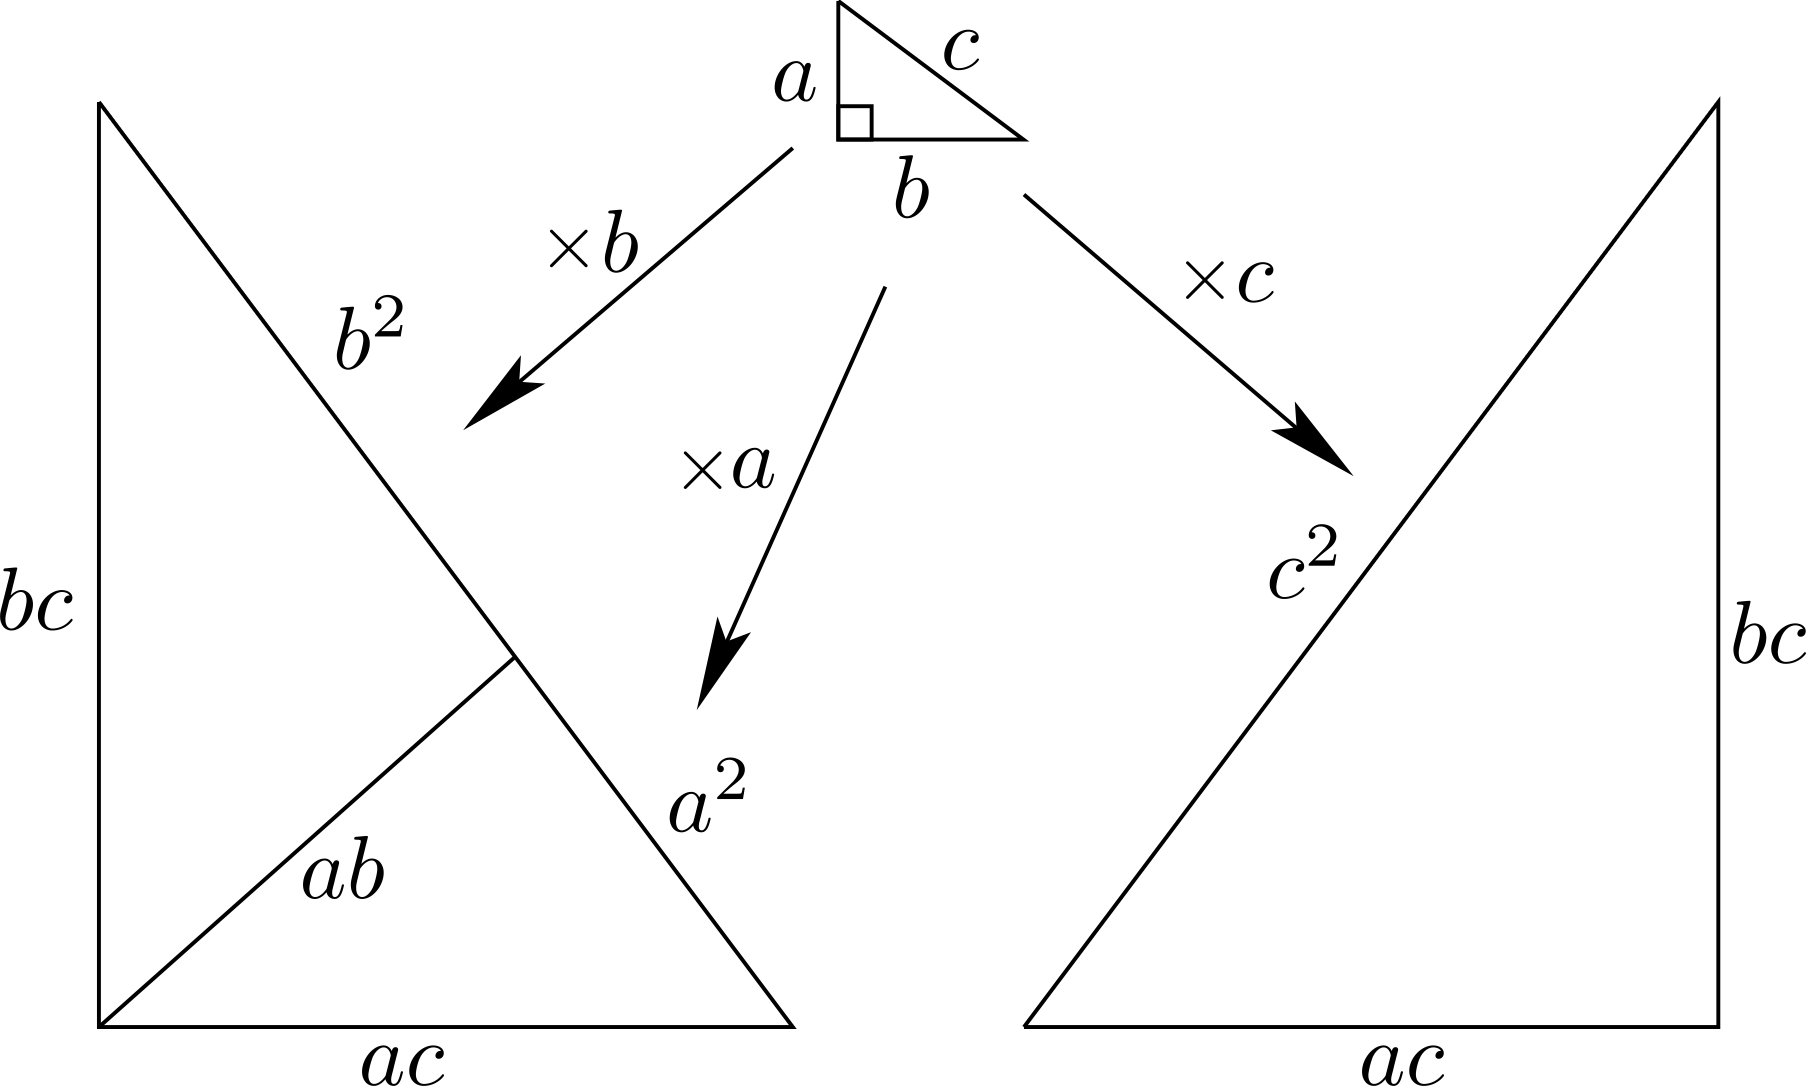
\includegraphics[scale=0.8]{pbpdilation.png}
\end{image}
\begin{freeResponse}
\end{freeResponse}
\begin{hint}
We are given a small right triangle with legs $a$ and $b$ and hypotenuse $c$.  We want to show that $a^2 + b^2 = c^2$.  

Sketch of proof:  The arrows represent scaling of that triangle by scale factors $b$, $a$, and $c$, resulting in three right triangles with side lengths as labeled.  The segments of length $a^2$ and $b^2$ are collinear (why?), which implies the two medium-sized triangles make a single large triangle on the left.  The large triangle on the left is a right triangle.  (Why?)  The two large triangles are congruent.  (Why?)  Then $a^2 + b^2 = c^2$.  (Why?)
\end{hint}
\end{question}

\end{document}
